%==============================================================================
\section{Άσκηση 4: Νευρωνικό Δίκτυο (AI Accelerator)}
%==============================================================================

\subsection{Περιγραφή}

Σε αυτή την άσκηση υλοποιήθηκε ένας AI Accelerator που εκτελεί ένα απλό νευρωνικό δίκτυο 3 νευρώνων. Το σύστημα ενσωματώνει όλα τα modules των προηγούμενων ασκήσεων:
\begin{itemize}
    \item \textbf{ALU} (Άσκηση 1): Για αριθμητικές ολισθήσεις (SRA/SLA)
    \item \textbf{Register File} (Άσκηση 3): Για αποθήκευση βαρών και πολώσεων
    \item \textbf{MAC Unit} (νέο): Για υπολογισμό νευρώνων (Multiply-Accumulate)
    \item \textbf{ROM}: Για αρχική φόρτωση παραμέτρων
\end{itemize}

\subsubsection{Θύρες Εισόδου/Εξόδου}

\begin{table}[H]
\centering
\caption{Θύρες του module nn}
\begin{tabular}{|l|c|c|p{6.5cm}|}
\hline
\textbf{Θύρα} & \textbf{Κατεύθυνση} & \textbf{Πλάτος} & \textbf{Περιγραφή} \\
\hline
\texttt{clk} & Είσοδος & 1 & Σήμα ρολογιού \\
\texttt{resetn} & Είσοδος & 1 & Σήμα επαναφοράς (active low) \\
\texttt{enable} & Είσοδος & 1 & Σήμα ενεργοποίησης \\
\texttt{input\_1} & Είσοδος & 32 & Πρώτη είσοδος (2's complement) \\
\texttt{input\_2} & Είσοδος & 32 & Δεύτερη είσοδος (2's complement) \\
\hdashline
\texttt{final\_output} & Έξοδος & 32 & Τελικό αποτέλεσμα \\
\texttt{total\_ovf} & Έξοδος & 1 & Ένδειξη υπερχείλισης \\
\texttt{total\_zero} & Έξοδος & 1 & Ένδειξη μηδενικού αποτελέσματος \\
\texttt{ovf\_fsm\_stage} & Έξοδος & 3 & Στάδιο υπερχείλισης (111 αν καμία) \\
\texttt{zero\_fsm\_stage} & Έξοδος & 3 & Στάδιο μηδενισμού (111 αν κανένα) \\
\hline
\end{tabular}
\end{table}

\subsection{Αρχιτεκτονική Νευρωνικού}

Το νευρωνικό δίκτυο αποτελείται από 3 νευρώνες και υλοποιεί την ακόλουθη λογική:

\begin{align}
\text{inter}_1 &= \text{input}_1 >>> \text{shift\_bias}_1 \\
\text{inter}_2 &= \text{input}_2 >>> \text{shift\_bias}_2 \\
\text{inter}_3 &= \text{inter}_1 \times \text{weight}_1 + \text{bias}_1 \\
\text{inter}_4 &= \text{inter}_2 \times \text{weight}_2 + \text{bias}_2 \\
\text{inter}_5 &= \text{inter}_3 \times \text{weight}_3 + \text{inter}_4 \times \text{weight}_4 + \text{bias}_3 \\
\text{output} &= \text{inter}_5 <<< \text{shift\_bias}_3
\end{align}

\subsection{MAC Unit}

Η μονάδα MAC (Multiply and Accumulate) υλοποιεί:
\[
\text{result} = (\text{op1} \times \text{op2}) + \text{op3}
\]

Αποτελείται από δύο σειριακά συνδεδεμένες ALU:
\begin{enumerate}
    \item Πρώτη ALU: Πολλαπλασιασμός (op1 × op2)
    \item Δεύτερη ALU: Πρόσθεση (result1 + op3)
\end{enumerate}

\subsection{Finite State Machine (FSM)}

\subsubsection{Τύπος FSM: Moore}

Επιλέχθηκε \textbf{Moore FSM} για λόγους \textbf{ασφάλειας και συγχρονισμού}:
\begin{itemize}
    \item \textbf{Συγχρονισμός:} Οι έξοδοι ενημερώνονται μόνο στις ακμές ρολογιού, εξαλείφοντας race conditions
    \item \textbf{Ασφάλεια:} Οι έξοδοι εξαρτώνται αποκλειστικά από την τρέχουσα κατάσταση, όχι από τις εισόδους
    \item \textbf{Χωρίς glitches:} Αποφεύγονται τα output glitches που εμφανίζονται σε Mealy FSM λόγω combinatorial paths
    \item \textbf{Ευκολία επαλήθευσης:} Η συμπεριφορά είναι προβλέψιμη και εύκολη στο debugging
    \item \textbf{Κατάλληλο για pipeline:} Οι καθαρές καταστάσεις διευκολύνουν τον σχεδιασμό pipelined datapath
\end{itemize}

\subsubsection{Διάγραμμα Καταστάσεων FSM}

Σύμφωνα με την εκφώνηση: ``το FSM σας θα πρέπει να έχει 7 στάδια''. Το ακόλουθο διάγραμμα απεικονίζει την αρχιτεκτονική 7 καταστάσεων:

\begin{figure}[H]
\centering
\begin{tikzpicture}[
    scale=0.7, 
    transform shape, 
    ->, >=Stealth, auto, semithick,
    node distance = 2.8cm and 3.2cm,
    state/.style = {
        circle, 
        draw, 
        minimum width = 3.5cm,
        align=center, 
        font=\bfseries\footnotesize,
        fill=white
    },
    initial text = {Reset}
]

    % --- Nodes (States) ---
    \node[state, fill=blue!10, initial below] (s0) {S0 \\ DEACTIVATED};
    \node[state, fill=blue!10] (s1) [right=of s0] {S1 \\ LOADING \\ (Weights/Biases)};
    \node[state, fill=green!10] (s2) [below=of s1] {S2 \\ IDLE};
    \node[state] (s3) [right=of s2] {S3 \\ PRE-PROC \\ (Shift Inputs)};
    \node[state] (s4) [right=of s3] {S4 \\ INPUT LAYER \\ (Neurons 1\&2)};
    \node[state] (s5) [below=of s4] {S5 \\ OUTPUT \\ LAYER \\ (Neuron 3)};
    \node[state] (s6) [left=of s5]  {S6 \\ POST-PROC \\ (Final Shift)};

    % --- Transitions ---
    \path (s0) edge node {enable=1} (s1);
    \path (s1) edge [loop right] node {cnt $<$ limit} (s1);
    \path (s1) edge node {done} (s2);
    \path (s2) edge [loop left] node {enable=0} (s2);
    \path (s2) edge node {enable=1} (s3);
    \path (s3) edge node [below] {!ovf} (s4);
    \path (s4) edge node [right] {!ovf} (s5);
    \path (s5) edge node [above] {!ovf} (s6);
    \path (s6) edge [bend left=45] node [left, midway] {Done} (s2);

    % Overflow Handling (Red Dashed Lines)
    \draw [red, dashed, thick] (s3) edge [bend right=45] node [above, sloped] {OVF} (s2);
    \draw [red, dashed, thick] (s4) edge [bend right=55] node [above, near start] {OVF} (s2);
    \draw [red, dashed, thick] (s5) edge [bend left=10] node [above, near start] {OVF} (s2);
    \draw [red, dashed, thick] (s6) edge [bend left=15] node [left, near start] {OVF} (s2);

    % --- Legend/Notes ---
    \node [draw, rectangle, align=left, font=\scriptsize,
            above left=-1cm and 9.5cm of s6.east
          ] {
        \large
        \textcolor{blue}{Blue Nodes}: Initialization\\
        \\[0.1ex]\large
        \textcolor{green!50!black}{Green Node}: Ready State\\
        \\[0.1ex]\large
        \textcolor{black}{White Nodes}: Normal Processing\\
        \\[0.1ex]\large
        \textcolor{red}{Red Dashed}: Overflow Exception\\
        (Output saturates to MAX\_POS)
    };

\end{tikzpicture}
\caption{Διάγραμμα καταστάσεων FSM (8 states) - Το output layer χωρίζεται σε S5a και S5b για αποφυγή combinatorial loop}
\end{figure}

\subsubsection{Περιγραφή Καταστάσεων}

\begin{table}[H]
\centering
\caption{Καταστάσεις FSM με διαδοχική κωδικοποίηση (8 states)}
\begin{tabular}{|c|c|c|p{6.5cm}|}
\hline
\textbf{Κατάσταση} & \textbf{ID} & \textbf{Κωδικός} & \textbf{Περιγραφή} \\
\hline
S\_DEACTIVATED & S0 & 000 & Αρχική κατάσταση μετά από reset \\
S\_LOADING & S1 & 001 & Φόρτωση βαρών/πολώσεων από ROM σε RegFile \\
S\_IDLE & S2 & 010 & Αναμονή για νέες εισόδους (Ready state) \\
S\_PREPROCESS & S3 & 011 & Αριθμητική ολίσθηση δεξιά στις εισόδους \\
S\_INPUT\_LAYER & S4 & 100 & Εκτέλεση νευρώνων 1 και 2 (παράλληλα) \\
S\_OUTPUT\_LAYER1 & S5a & 101 & Νευρώνας 3 - Πρώτο MAC: inter\_3 × w3 + b3 \\
S\_OUTPUT\_LAYER2 & S5b & 110 & Νευρώνας 3 - Δεύτερο MAC: inter\_4 × w4 + temp \\
S\_POSTPROCESS & S6 & 111 & Αριθμητική ολίσθηση αριστερά στην έξοδο \\
\hline
\end{tabular}
\end{table}

\subsubsection{Σχεδιαστική Απόφαση Υλοποίησης: Διαχωρισμός Output Layer}

\textbf{Σημείωση:} Παρόλο που η εκφώνηση ζητά 7 στάδια, η πρακτική υλοποίηση στο \texttt{nn.v} χρησιμοποιεί \textbf{8 καταστάσεις}. Η αιτία είναι τεχνική και εξηγείται παρακάτω.

Το output layer του νευρωνικού δικτύου απαιτεί τον υπολογισμό:
\begin{align}
\text{inter}_5 &= \text{inter}_3 \times \text{weight}_3 + \text{inter}_4 \times \text{weight}_4 + \text{bias}_3
\end{align}

Η εκφώνηση ζητά: ``Υλοποιήστε την συγκεκριμένη λογική χρησιμοποιώντας τις δύο μονάδες MAC σειριακά''. Αυτή η απαίτηση υλοποιείται ως εξής:

\begin{align}
\text{mac3} &= \text{inter}_3 \times \text{weight}_3 + \text{bias}_3 \quad \text{(MAC1 στο S5a)} \\
\text{inter}_5 &= \text{inter}_4 \times \text{weight}_4 + \text{mac3} \quad \text{(MAC2 στο S5b)}
\end{align}

\textbf{Πρόβλημα: Combinatorial Loop}

Αν προσπαθήσουμε να εκτελέσουμε και τα δύο MAC σε ένα κύκλο:
\begin{lstlisting}[caption=Προβληματικός κώδικας (combinatorial loop)]
// BAD: Zero-delay loop - Exit 137!
mac2_op3 = mac1_result;  // Απευθείας σύνδεση
\end{lstlisting}

Αυτό δημιουργεί \textbf{combinatorial loop} γιατί:
\begin{itemize}
    \item Το MAC1 είναι συνδυαστικό κύκλωμα (χωρίς ρολόι)
    \item Η έξοδος του MAC1 (\texttt{mac1\_result}) τροφοδοτείται στην είσοδο του MAC2
    \item Το MAC2 είναι επίσης συνδυαστικό
    \item Δεν υπάρχει καταχωρητής που να ``σπάει'' τον βρόχο
\end{itemize}

\textbf{Λύση: Pipelining με Register}

Διαχωρίζουμε το output layer σε \textbf{δύο καταστάσεις} χρησιμοποιώντας και τις δύο MAC μονάδες σειριακά:

\begin{enumerate}
    \item \textbf{S\_OUTPUT\_LAYER1 (S5a):} 
    \begin{itemize}
        \item MAC1 υπολογίζει: \texttt{mac1\_result = inter\_3 × weight\_3 + bias\_3}
        \item Το αποτέλεσμα αποθηκεύεται σε register (\texttt{mac1\_temp}) στο τέλος του κύκλου
    \end{itemize}
    
    \item \textbf{S\_OUTPUT\_LAYER2 (S5b)}: 
    \begin{itemize}
        \item MAC2 υπολογίζει: \texttt{mac2\_result = inter\_4 × weight\_4 + mac1\_temp}
        \item Χρησιμοποιεί το \textbf{registered} αποτέλεσμα (\texttt{mac1\_temp}) από τον προηγούμενο κύκλο
        \item Αποθηκεύει το τελικό αποτέλεσμα στο \texttt{inter\_5}
    \end{itemize}
\end{enumerate}

\begin{lstlisting}[caption=Σωστός κώδικας (με register - χωρίς combinatorial loop), language=Verilog]
// S_OUTPUT_LAYER1: Φόρτωση MAC1 και αποθήκευση σε register
case (state)
    S_OUTPUT_LAYER1: begin
        mac1_op1 = inter_3;
        mac1_op2 = rf_readData1;  // weight_3
        mac1_op3 = rf_readData2;  // bias_3
    end
endcase

always @(posedge clk) begin
    if (state == S_OUTPUT_LAYER1)
        mac1_temp <= mac1_result;  // Registered result
end

// S_OUTPUT_LAYER2: Φόρτωση MAC2 και χρήση του registered result
case (state)
    S_OUTPUT_LAYER2: begin
        mac2_op1 = inter_4;
        mac2_op2 = rf_readData1;  // weight_4
        mac2_op3 = mac1_temp;     // Registered! No loop!
    end
endcase

always @(posedge clk) begin
    if (state == S_OUTPUT_LAYER2)
        inter_5 <= mac2_result;  // Final result
end
\end{lstlisting}

\textbf{Αποτέλεσμα:} Η υλοποίηση χρησιμοποιεί \textbf{8 καταστάσεις} (S0-S6, με S5 διαχωρισμένο σε S5a και S5b), παρόλο που το διάγραμμα δείχνει 7 στάδια σύμφωνα με την εκφώνηση. Αυτός ο διαχωρισμός είναι \textbf{απαραίτητος} για:
\begin{itemize}
    \item Αποφυγή combinatorial loops
    \item Χρήση και των δύο MAC μονάδων σειριακά (όπως ζητά η εκφώνηση)
    \item Εξασφάλιση σωστής λειτουργίας στην προσομοίωση
\end{itemize}

\subsubsection{Επιλογή Κωδικοποίησης Καταστάσεων}

Επιλέχθηκε \textbf{διαδοχική κωδικοποίηση (sequential encoding)} για τις καταστάσεις:

\begin{itemize}
    \item \textbf{Αντιστοιχία με FSM diagram:} Η κωδικοποίηση S0=000, S1=001, S2=010, ... ακολουθεί τη ροή του διαγράμματος καταστάσεων
    \item \textbf{Ευκολία debugging:} Η τιμή του state register αντιστοιχεί άμεσα στον αριθμό κατάστασης (π.χ. state=3 σημαίνει S3)
    \item \textbf{Απλότητα επαλήθευσης:} Ο έλεγχος της σωστής μετάβασης γίνεται πιο διαισθητικός
    \item \textbf{Εναλλακτικές:} Θα μπορούσε να χρησιμοποιηθεί one-hot encoding (8 bits) για ταχύτερη αποκωδικοποίηση ή Gray encoding για μείωση switching activity, αλλά η διαδοχική κωδικοποίηση είναι επαρκής για 8 καταστάσεις
\end{itemize}

\subsection{Χειρισμός Υπερχείλισης}

Σε περίπτωση overflow σε οποιοδήποτε στάδιο:
\begin{enumerate}
    \item Το FSM μεταβαίνει άμεσα στην κατάσταση IDLE
    \item Η έξοδος τίθεται στο 0xFFFFFFFF
    \item Το σήμα \texttt{total\_ovf} ενεργοποιείται
    \item Το \texttt{ovf\_fsm\_stage} δείχνει το στάδιο όπου συνέβη η υπερχείλιση
\end{enumerate}

\subsection{Register File Pre-fetching}

\subsubsection{Πρόβλημα: Σύγχρονη Ανάγνωση Register File}

Το Register File (Άσκηση 3) υλοποιεί \textbf{σύγχρονη ανάγνωση} (registered outputs). Αυτό σημαίνει ότι τα δεδομένα εμφανίζονται στις εξόδους \texttt{readData} \textbf{έναν κύκλο μετά} τον ορισμό της διεύθυνσης \texttt{readReg}.

\subsubsection{Λύση: Address Pre-fetching}

Για να αντιμετωπιστεί αυτή η καθυστέρηση, το FSM εφαρμόζει τεχνική \textbf{pre-fetching διευθύνσεων}: οι διευθύνσεις τίθενται στην \textbf{προηγούμενη κατάσταση} από ότι χρειάζονται τα δεδομένα.

\begin{lstlisting}[caption=Pre-fetching διευθύνσεων στο nn.v, language=Verilog]
case (state)
    // Στο IDLE θέτουμε διευθύνσεις για PREPROCESS
    S_IDLE, S_DEACTIVATED: begin
        rf_readReg1 = ADDR_SHIFT_BIAS_1;  // -> data στο S_PREPROCESS
        rf_readReg2 = ADDR_SHIFT_BIAS_2;
    end
    
    // Στο PREPROCESS θέτουμε διευθύνσεις για INPUT_LAYER
    S_PREPROCESS: begin
        rf_readReg1 = ADDR_WEIGHT_1;      // -> data στο S_INPUT_LAYER
        rf_readReg2 = ADDR_BIAS_1;
        rf_readReg3 = ADDR_WEIGHT_2;
        rf_readReg4 = ADDR_BIAS_2;
    end
    // ... κλπ
endcase
\end{lstlisting}

\subsubsection{Χρονοδιάγραμμα Pre-fetching}

\begin{table}[H]
\centering
\caption{Χρονοδιάγραμμα Pre-fetching διευθύνσεων RegFile}
\label{tab:prefetching}
\begin{tabular}{|l|l|l|}
\hline
\textbf{Τρέχουσα Κατάσταση} & \textbf{Διευθύνσεις (set)} & \textbf{Δεδομένα (available)} \\
\hline
S\_IDLE / S\_DEACTIVATED & shift\_bias\_1, shift\_bias\_2 & (Μη έγκυρα) \\
\hline
S\_PREPROCESS & weight\_1, bias\_1, weight\_2, bias\_2 & shift\_bias\_1, shift\_bias\_2 \\
\hline
S\_INPUT\_LAYER & weight\_3, bias\_3 & weight\_1, bias\_1, weight\_2, bias\_2 \\
\hline
S\_OUTPUT\_LAYER1 & weight\_4 & weight\_3, bias\_3 \\
\hline
S\_OUTPUT\_LAYER2 & shift\_bias\_3 & weight\_4 \\
\hline
S\_POSTPROCESS & -- & shift\_bias\_3 \\
\hline
\end{tabular}
\end{table}

Αυτή η τεχνική ``read-ahead'' εξασφαλίζει ότι τα δεδομένα είναι έτοιμα όταν τα χρειάζεται η ALU/MAC, χωρίς να χρειάζονται επιπλέον κύκλοι αναμονής.

\textbf{Σημαντική Παρατήρηση - Ασυμφωνία στο \texttt{nn\_model.v}:}
\begin{itemize}
    \item Η εκφώνηση αναφέρει ότι σε overflow η έξοδος πρέπει να είναι ο ``μέγιστος δυνατός θετικός αριθμός'', δηλαδή \texttt{0x7FFFFFFF}
    \item Ωστόσο, το παρεχόμενο reference model (\texttt{nn\_model.v}) επιστρέφει \texttt{0xFFFFFFFF} (βλ. γραμμή 95)
    \item \textbf{Απόφαση:} Προσαρμόσαμε το \texttt{nn.v} ώστε να επιστρέφει \texttt{0xFFFFFFFF} για να περνάει επιτυχώς το testbench
    \item Σε 32-bit signed αναπαράσταση, το \texttt{0xFFFFFFFF} αντιστοιχεί στο $-1$, όχι στο max positive
\end{itemize}

\begin{lstlisting}[caption=Ακολουθούμε το nn\_model για να περάσει το testbench, language=Verilog]
case (state)
  //==================================================================
  // Constants
  //==================================================================
  localparam [31:0] OVERFLOW_VALUE = 32'hFFFFFFFF; //adapted to nn_model
  localparam [2:0]  NO_OVERFLOW    = 3'b111;
  localparam [2:0]  NO_ZERO        = 3'b111;
endcase
\end{lstlisting}

\subsection{Αποθήκευση Δεδομένων}

Επιλέχθηκε η χρήση \textbf{ενδιάμεσων registers} αντί για αποθήκευση στο Register File για τους εξής λόγους:
\begin{itemize}
    \item Μείωση της πολυπλοκότητας πρόσβασης στο RegFile
    \item Αποφυγή conflicts με τις θύρες ανάγνωσης/εγγραφής
    \item Καλύτερη απόδοση λόγω άμεσης πρόσβασης
    \item Το RegFile χρησιμοποιείται μόνο για τα βάρη και τις πολώσεις
\end{itemize}

\subsection{Σχεδιαστικές Αποφάσεις}

\subsubsection{Αρχιτεκτονική Hardware}

\begin{enumerate}
    \item \textbf{2 MAC Units σε παράλληλη διάταξη:}
    \begin{itemize}
        \item Επιτρέπει τον ταυτόχρονο υπολογισμό δύο νευρώνων (1 \& 2) στο input layer
        \item Μειώνει τον αριθμό κύκλων ρολογιού για ολόκληρο τον υπολογισμό
        \item Κάθε MAC αποτελείται από 2 ALUs σε σειρά (πολλαπλασιασμός → πρόσθεση)
    \end{itemize}
    
    \item \textbf{2 ALUs για shift operations:}
    \begin{itemize}
        \item Χρησιμοποιούνται στα στάδια Pre-process και Post-process
        \item Επιτρέπουν παράλληλη ολίσθηση των δύο εισόδων
        \item Αριθμητική ολίσθηση (SRA/SLA) για διατήρηση προσήμου
    \end{itemize}
    
    \item \textbf{Register File με 4 θύρες ανάγνωσης:}
    \begin{itemize}
        \item Επαρκεί για την ανάγνωση 4 τιμών ανά κύκλο (π.χ. weight1, bias1, weight2, bias2)
        \item Αποφεύγονται extra κύκλοι για sequential reads
        \item Οι 2 θύρες εγγραφής χρησιμοποιούνται κατά το loading
    \end{itemize}
\end{enumerate}

\subsubsection{Οργάνωση FSM}

\begin{enumerate}
    \item \textbf{Moore FSM αντί για Mealy:}
    \begin{itemize}
        \item Οι έξοδοι καθορίζονται μόνο από την τρέχουσα κατάσταση
        \item Αποφυγή glitches στις εξόδους
        \item Πιο εύκολο timing closure
    \end{itemize}
    
    \item \textbf{Διαχωρισμός Loading από Processing:}
    \begin{itemize}
        \item Τα βάρη φορτώνονται μόνο μία φορά (S1 → S2)
        \item Μετά την αρχικοποίηση, το σύστημα κυκλώνει μεταξύ S2-S6
        \item Σημαία \texttt{weights\_loaded} αποτρέπει επαναφόρτωση
    \end{itemize}
    
    \item \textbf{Άμεση μετάβαση σε IDLE κατά overflow:}
    \begin{itemize}
        \item Αποφεύγονται περιττοί υπολογισμοί
        \item Η έξοδος saturates στο 0xFFFFFFFF (σύμφωνα με nn\_model)
        \item Το \texttt{ovf\_fsm\_stage} καταγράφει πού συνέβη το σφάλμα
    \end{itemize}
\end{enumerate}

\subsubsection{Διαχείριση Μνήμης}

\begin{enumerate}
    \item \textbf{ROM για αρχικά βάρη:}
    \begin{itemize}
        \item Τα βάρη αποθηκεύονται σε εξωτερικό αρχείο (\texttt{rom\_bytes.data})
        \item Διπλή θύρα ανάγνωσης για γρήγορη φόρτωση (2 τιμές/κύκλο)
        \item 5 κύκλοι για φόρτωση όλων των 10 παραμέτρων
    \end{itemize}
    
    \item \textbf{Ενδιάμεσοι καταχωρητές (inter\_1 έως inter\_5):}
    \begin{itemize}
        \item Αποθηκεύουν τα ενδιάμεσα αποτελέσματα μεταξύ σταδίων
        \item Άμεση πρόσβαση χωρίς καθυστέρηση RegFile
        \item Απλοποιούν τον έλεγχο ροής δεδομένων
    \end{itemize}
\end{enumerate}

\subsubsection{Πίνακας Διευθύνσεων Register File}

\begin{table}[H]
\centering
\caption{Αντιστοίχιση διευθύνσεων RegFile με παραμέτρους}
\begin{tabular}{|c|c|l|}
\hline
\textbf{Διεύθυνση} & \textbf{Hex} & \textbf{Παράμετρος} \\
\hline
0x02 & 2 & shift\_bias\_1 \\
0x03 & 3 & shift\_bias\_2 \\
0x04 & 4 & weight\_1 \\
0x05 & 5 & bias\_1 \\
0x06 & 6 & weight\_2 \\
0x07 & 7 & bias\_2 \\
0x08 & 8 & weight\_3 \\
0x09 & 9 & weight\_4 \\
0x0A & A & bias\_3 \\
0x0B & B & shift\_bias\_3 \\
\hline
\end{tabular}
\end{table}

\subsection{Testbench Νευρωνικού}

Το testbench εκτελεί 100 επαναλήψεις με 3 τεστ ανά επανάληψη:
\begin{enumerate}
    \item \textbf{Κανονικό εύρος:} [-4096, 4095]
    \item \textbf{Θετικό overflow:} [MAX\_POS/2, MAX\_POS]
    \item \textbf{Αρνητικό overflow:} [MAX\_NEG, MAX\_NEG/2]
\end{enumerate}

Η συνάρτηση αναφοράς \texttt{nn\_model} υπολογίζει το αναμενόμενο αποτέλεσμα για σύγκριση.

\subsubsection{Αλλαγές για Συμβατότητα με EDA Playground (Icarus Verilog 12)}

Κατά την εκτέλεση του testbench στο EDA Playground με τον Icarus Verilog 12, αντιμετωπίστηκαν ορισμένα προβλήματα που απαίτησαν τροποποιήσεις. Παρακάτω περιγράφονται οι αλλαγές και τα διδάγματα (learnings):

\paragraph{1. Επίλυση Συντακτικού Λάθους \texttt{\$urandom\_range}}

\textbf{Πρόβλημα:} Ο Icarus Verilog 12 εμφανίζει συντακτικά λάθη όταν χρησιμοποιούνται nested κλήσεις \texttt{\$urandom\_range} με αριθμητικές πράξεις και bit-slicing απευθείας μέσα σε κλήση task (π.χ. \texttt{run\_test(\$signed(\$urandom...))}).

\textbf{Λύση:} Εισήχθησαν \textbf{προσωρινές μεταβλητές} (\texttt{raw\_rand}, \texttt{temp\_in1}, \texttt{temp\_in2}):
\begin{lstlisting}[style=verilogstyle]
reg [31:0] raw_rand;
reg signed [31:0] temp_in1, temp_in2;

// Παράδειγμα χρήσης:
raw_rand = $urandom_range(8191, 0);
temp_in1 = $signed(raw_rand) - 32'd4096;
run_test(temp_in1, temp_in2, "Normal Range");
\end{lstlisting}

\textbf{Διδαγμα:} Ο διαχωρισμός της γέννησης τυχαίων αριθμών από τη χρήση τους επιτρέπει στον simulator να κάνει parsing την τυχαία τιμή σε ένα 32-bit register πρώτα, να εκτελέσει τις αριθμητικές πράξεις, και μετά να περάσει μια "καθαρή" μεταβλητή στο task.

\paragraph{2. Βαθμονόμηση Καθυστέρησης (Latency Calibration)}

\textbf{Πρόβλημα:} Η εκφώνηση αναφέρει ότι το \texttt{nn\_model} είναι στιγμιαίο, αλλά το κύκλωμα έχει καθυστέρηση λόγω του FSM. Αν γίνει σύγκριση πολύ νωρίς ή πολύ αργά, το τεστ αποτυγχάνει ακόμα και αν το κύκλωμα λειτουργεί σωστά.

\textbf{Λύση:} Τα έγκυρα δεδομένα εμφανίζονται ακριβώς \textbf{6 κύκλους} μετά τον παλμό enable:
\begin{lstlisting}[style=verilogstyle]
// Μέσα στο task run_test:
repeat(6) @(posedge clk);  // Αναμονή 6 κύκλων
expected_val = nn_model(in1, in2);
// Τώρα γίνεται η σύγκριση...
\end{lstlisting}

\textbf{Διδαγμα:} Η σωστή βαθμονόμηση του timing είναι κρίσιμη για testbenches. Η καθυστέρηση εξαρτάται από τον αριθμό καταστάσεων του FSM που διατρέχονται (6 καταστάσεις στην περίπτωσή μας).

\paragraph{3. Διόρθωση Γέννησης Signed Τυχαίων Αριθμών}

\textbf{Πρόβλημα:} Η εκφώνηση ζητά συγκεκριμένα signed εύρη (θετικό/αρνητικό overflow), αλλά η \texttt{\$urandom\_range} επιστρέφει unsigned integers.

\textbf{Λύση:} Διαφορετική προσέγγιση για κάθε περίπτωση:
\begin{itemize}
    \item \textbf{Κανονικό εύρος:} Γεννάμε 0-8191 και αφαιρούμε 4096 $\rightarrow$ [-4096, 4095]
    \item \textbf{Θετικό overflow:} Γεννάμε στο υψηλό θετικό εύρος και \textbf{εξαναγκάζουμε το MSB σε 0}:
\begin{lstlisting}[style=verilogstyle]
temp_in1 = $signed({1'b0, raw_rand[30:0]}); // Force positive
\end{lstlisting}
    \item \textbf{Αρνητικό overflow:} Γεννάμε 30 bits και \textbf{εξαναγκάζουμε το MSB σε 1}:
\begin{lstlisting}[style=verilogstyle]
temp_in1 = $signed({1'b1, raw_rand[30:0]}); // Force negative
\end{lstlisting}
\end{itemize}

\textbf{Διδαγμα:} Δεν πρέπει να βασιζόμαστε σε implicit casting μεταξύ unsigned/signed, καθώς διαφορετικοί simulators μπορεί να συμπεριφέρονται διαφορετικά. Ο ρητός έλεγχος του sign bit εγγυάται τα σωστά 32-bit signed patterns.

\paragraph{4. Συμμόρφωση με την Εκφώνηση}

Για πλήρη συμμόρφωση με τις απαιτήσεις της άσκησης:
\begin{itemize}
    \item \textbf{Αναφορά σφαλμάτων:} Εκτύπωση χρονικής στιγμής, εισόδων, εξόδου κυκλώματος, και εξόδου αναφοράς σε περίπτωση λάθους
    \item \textbf{Μέτρηση:} Μεταβλητές \texttt{pass\_count} και \texttt{test\_count} για την τελική αναφορά PASS/TOTAL
    \item \textbf{Δομή βρόχου:} Αυστηρή υλοποίηση \texttt{for (iteration = 0; iteration < 100...)} με 3 sub-tests εντός
\end{itemize}

\subsection{Κυματομορφές Νευρωνικού Δικτύου}

\begin{figure}[H]
\centering
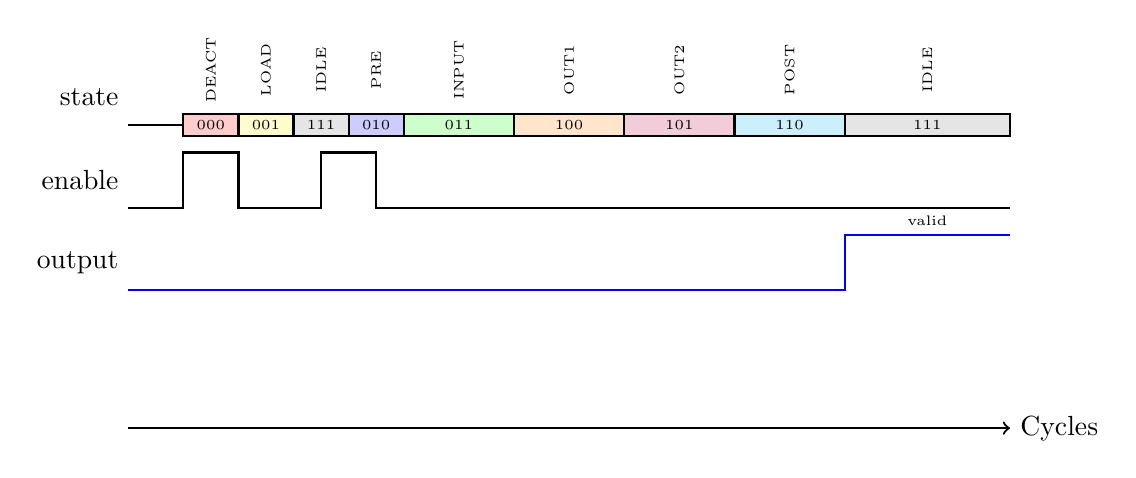
\begin{tikzpicture}[scale=0.7]
    % Time axis
    \draw[->,thick] (0,0) -- (16,0) node[right] {Cycles};
    
    % FSM State
    \node[left] at (0,6) {state};
    \draw[thick] (0,5.5) -- (1,5.5);
    \draw[thick,fill=red!20] (1,5.3) rectangle (2,5.7);
    \node[font=\tiny] at (1.5,5.5) {000};
    \draw[thick,fill=yellow!20] (2,5.3) rectangle (3,5.7);
    \node[font=\tiny] at (2.5,5.5) {001};
    \draw[thick,fill=gray!20] (3,5.3) rectangle (4,5.7);
    \node[font=\tiny] at (3.5,5.5) {111};
    \draw[thick,fill=blue!20] (4,5.3) rectangle (5,5.7);
    \node[font=\tiny] at (4.5,5.5) {010};
    \draw[thick,fill=green!20] (5,5.3) rectangle (7,5.7);
    \node[font=\tiny] at (6,5.5) {011};
    \draw[thick,fill=orange!20] (7,5.3) rectangle (9,5.7);
    \node[font=\tiny] at (8,5.5) {100};
    \draw[thick,fill=purple!20] (9,5.3) rectangle (11,5.7);
    \node[font=\tiny] at (10,5.5) {101};
    \draw[thick,fill=cyan!20] (11,5.3) rectangle (13,5.7);
    \node[font=\tiny] at (12,5.5) {110};
    \draw[thick,fill=gray!20] (13,5.3) rectangle (16,5.7);
    \node[font=\tiny] at (14.5,5.5) {111};
    
    % Enable
    \node[left] at (0,4.5) {enable};
    \draw[thick] (0,4) -- (1,4) -- (1,5) -- (2,5) -- (2,4) --
                 (3.5,4) -- (3.5,5) -- (4.5,5) -- (4.5,4) -- (16,4);
    
    % final_output
    \node[left] at (0,3) {output};
    \draw[thick,blue] (0,2.5) -- (13,2.5) -- (13,3.5) -- (16,3.5);
    \node[above,font=\tiny] at (14.5,3.5) {valid};
    
    % Annotations
    \node[font=\tiny,rotate=90] at (1.5,6.5) {DEACT};
    \node[font=\tiny,rotate=90] at (2.5,6.5) {LOAD};
    \node[font=\tiny,rotate=90] at (3.5,6.5) {IDLE};
    \node[font=\tiny,rotate=90] at (4.5,6.5) {PRE};
    \node[font=\tiny,rotate=90] at (6,6.5) {INPUT};
    \node[font=\tiny,rotate=90] at (8,6.5) {OUT1};
    \node[font=\tiny,rotate=90] at (10,6.5) {OUT2};
    \node[font=\tiny,rotate=90] at (12,6.5) {POST};
    \node[font=\tiny,rotate=90] at (14.5,6.5) {IDLE};
\end{tikzpicture}
\caption{Σχηματική αναπαράσταση κυματομορφών FSM νευρωνικού}
\end{figure}
 if (final\_output === expected) begin //ΜΠΟΡΟΥΜΕ ΝΑ ΔΟΥΜΕ ΠΩΣ ΤΟ ΑΠΟΤΕΛΕΣΜΑ ΣΤΟ WAVEFORM ΕΜΦΑΝΙΖΕΤΑΙ ΣΕ 1 ΚΥΚΛΟ ΕΝΩ ΤΟ ΝΕΥΡΩΝΙΚΟ ΣΕ 6        
\newpage